\subsection{Input problem}\label{ssec:boulder}
The input vector consists of a $5x5$ grid of bipolar values. The network is capable of classifying
input grids representing the $5$ vowels of the English alphabet, as shown in Figure
\ref{fig:charsIn}.

\begin{figure*}
    \centering
    \subfigure[Vowel A]{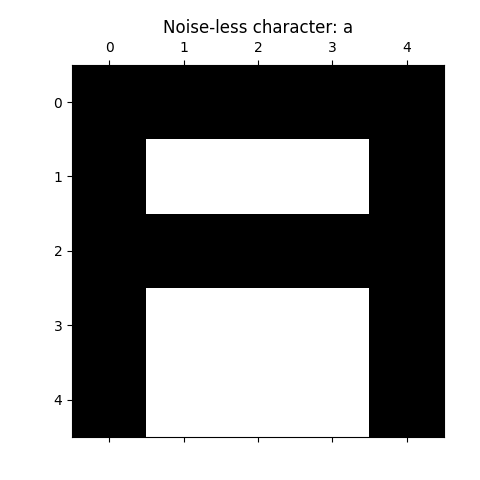
\includegraphics[width=0.18\textwidth]{images/vanilla_a.png}}
    \subfigure[Vowel E]{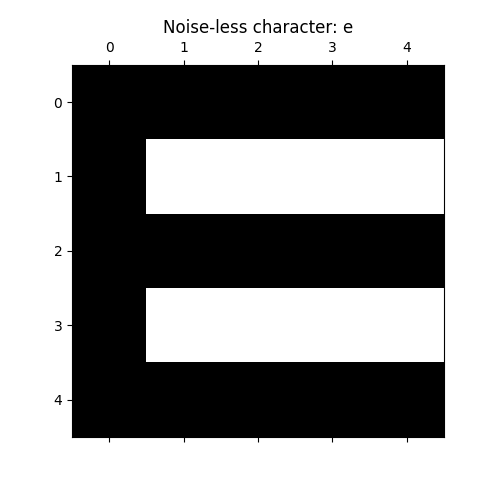
\includegraphics[width=0.18\textwidth]{images/vanilla_e.png}}
    \subfigure[Vowel I]{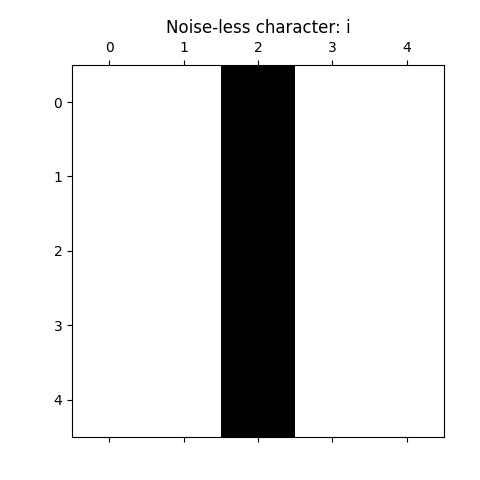
\includegraphics[width=0.18\textwidth]{images/vanilla_i.png}}
    \subfigure[Vowel O]{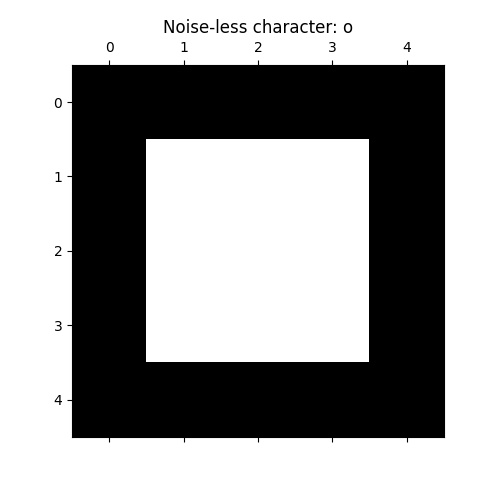
\includegraphics[width=0.18\textwidth]{images/vanilla_o.png}}
    \subfigure[Vowel U]{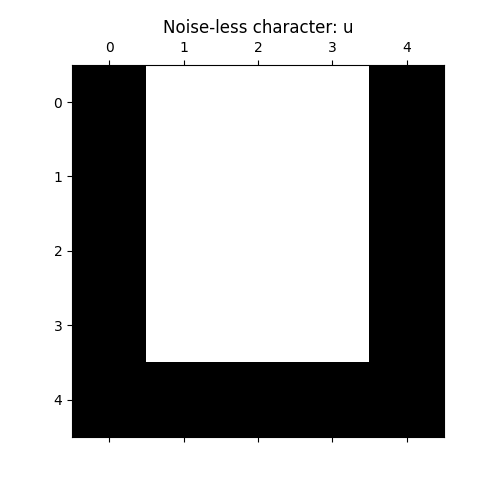
\includegraphics[width=0.18\textwidth]{images/vanilla_u.png}}
    \label{fig:charsIn}
    \caption{Input problem and recognizable vowels}
\end{figure*}

\begin{figure*}
    \centering
    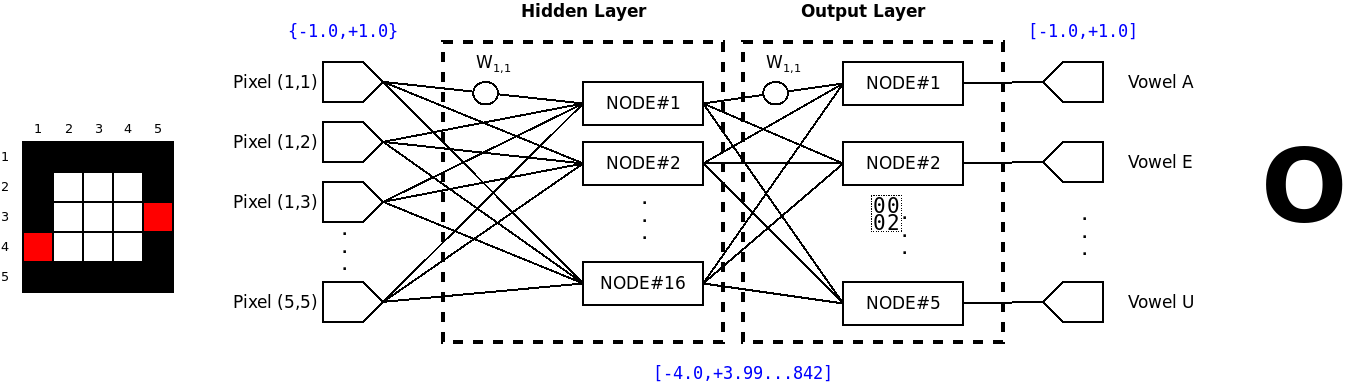
\includegraphics[width=\textwidth]{images/Architecture.png}
    \label{fig:netArchi}
    \caption{Architecture of the Neural Network}
\end{figure*}
The architecture of the designed Neural Network is shown in Figure \ref{fig:netArchi}. At the
highest level the network behaves as a Madaline network \cite{23872}, in that inputs and outputs
take bipolar values in the ${-1.0, 1.0}$ set. However, the internals of the network work with
fractional values, i.e. fixed-point values bounded to the $[-1.0,1.0]$ range.

The network is composed of two layers. An Input Layer connects $25$ inputs to $16$ neurons. An
Output Layer connects $16$ neurons to $5$ output nodes. Pixels from the $5x5$ input grid are all
mapped to inputs, while the output vector encodes the prediction as one-hot. Input and Output layer
are both fully connected.

recognized. All $25$ pixels take values in the ${-1.0,1.0}$ set, corresponding to the white
respectively dark pixels in the image. Up to $3$ noisy pixels are covered. A noisy pixel (shown in
red in Figure \ref{fig:netArchi}) is one that inverts its value from the original specification
found in Figure \ref{fig:charsIn}.
